\section{Semantic Web}
In 2001 heeft Tim Berners-Lee (uitvinder van het World Wide Web) het over een nieuwe revolutie. Dit is de eerste introductie van het \textit{Semantic Web} (soms wordt er ook naar verwezen onder de term \textit{Web 3.0}). Hierbij zou het web zoals het toen was evolueren. Zo is het web altijd leesbaar geweest voor mensen, maar niet interpreteerbaar door machines. Het \textit{Semantic Web} zou hier verandering in brengen. Zo zouden machines het web op dezelfde manier kunnen interpreteren zoals mensen dat doen. Deze machines heten \textit{intelligent agents} en zij zouden complexe taken volledig autonoom kunnen uitvoeren \cite{berners2001semantic}.

Om dit mogelijk te maken zijn er verschillende stappen nodig. Als eerste moet er voor gezorgd worden dat er betekenis gegeven kan worden op een manier die computers kunnen begrijpen. Ook is het belangrijk dat deze kennis gerepresenteerd kan worden aan de machines. Zo wordt er gebruik gemaakt van het RDF model (zie \sectionref{sec:rdf}) met behulp van bijvoorbeeld XML. Verder is het ook belangrijk om er rekening mee te houden dat informatie uit verschillende databanken een andere terminologie kan gebruiken om hetzelfde uit te drukken. Hiervoor wordt gebruik gemaakt van verschillende ontologieën (een definitie van de term ontologie wordt gegeven in \subsubsectionref{subsubsec:ontology}). De echte kracht van het \textit{Semantic Web} zal komen wanneer programma's gemaakt worden die informatie verzamelen van verschillende bronnen (de zogenaamde \textit{intelligent agent}) \cite{berners2001semantic}.

Een belangrijk aspect om het \textit{Semantic Web} mogelijk te maken is dus decentralisatie. Hiermee wordt bedoeld dat de macht (hier in de vorm van informatie) niet in handen mag zijn van enkele grote spelers, maar verspreid moet worden. In een ideale vorm van het \textit{Semantic Web} zou elke persoon een \textit{pod} hebben die de informatie over zichzelf bevat. Wanneer een website toegang tot deze informatie zou willen, dan zou deze informatie uit de \textit{pod} opgehaald moeten worden. Dit zou nog andere voordelen brengen, zoals onder andere een verbeterde privacy (toegang verlenen aan wie de persoon wil).

\subsection{Semantic Web Stack}
Het is vanzelfsprekend dat de architectuur van het \textit{Semantic Web} gebaseerd is op een hiërarchie van talen, waarbij elke taal de mogelijkheden van de talen lager in deze hiërarchie optimaal zal benutten en uitbreiden. Deze hiërarchie is gevisualiseerd in \figureref{fig:semantic_web_stack}, ontworpen door Tim Berners-Lee. In de paper ``Semantic Web Architecture: Stack or Two Towers?'' worden alternatieve voorstellingen van de \textit{Semantic Web Stack} besproken \cite{horrocks2005semantic}. In deze scriptie wordt niet verder ingegaan op deze uitbreidingen. De lagen van de oorspronkelijke \textit{Semantic Web Stack} die belangrijk zijn voor deze scriptie, worden hieronder besproken.

\begin{figure}[ht]
    \centering
    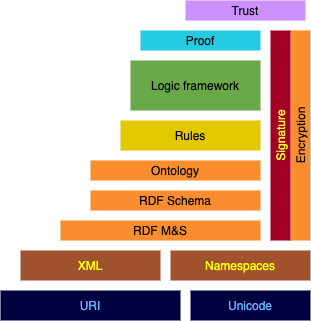
\includegraphics[width=0.5\linewidth]{images/Semantic Web Stack.png}
    \caption{Semantic Web Stack (gebaseerd op \textit{Semantic Web Stack} \cite{semanticwebstack})}
    \label{fig:semantic_web_stack}
\end{figure}

\subsubsection{Unicode}
Unicode is een systeem voor het encoderen van karakters. Net zoals ASCII is het ontwikkeld met het doel om ontwikkelaars te ondersteunen in het maken van applicaties. Unicode pakt de problemen aan van eerdere karakter encodeer systemen, zoals onder het niet ondersteunen van alle karakters. Zo zal unicode een uniek nummer hebben voor elk karakter op elk platform, voor elk programma en in elke taal \cite{unicode}.

Unicode ligt aan de basis van de \textit{Semantic Web Stack} omdat het \textit{Semantic Web} documenten in verschillende talen moet kunnen doorgeven. Deze documenten moeten dus ook kunnen gerepresenteerd worden.

\subsubsection{URI}
URI staat voor \textit{Uniform Resource Identifier}. Dit is dus een uniforme manier voor het identificeren van objecten. Deze term wordt soms door elkaar gehaald met de term URL, wat staat voor \textit{Uniform Resource Locator}. Het grote verschil tussen beide is dat een URI een object kan identificeren (= hoe iets te benoemen), terwijl een URL een object kan localiseren (= waar iets te vinden). De verwarring tussen beide komt door de onderlinge relatie tussen beide. Om dit verschil te begrijpen is het belangrijk te weten dat de verzameling van URL's een subset is van alle URI's. Zo is elke URL een URI, maar niet omgekeerd \cite{uri}.

Naast unicode ligt URI mede aan de basis van de \textit{Semantic Web Stack} omdat deze het mogelijk maken om op het Web resources te identificeren op eenzelfde eenvoudige manier.

\subsubsection{XML}
XML staat voor \textit{Extensible Markup Language}. Het wordt gebruikt voor de beschrijving van data. Eén van de belangrijkste kenmerken van de XML standaard is dat deze op een zeer flexibele manier data kan structureren. Het W3C beveelt XML dan ook aan. XML werkt aan de hand van elementen die gedefinieerd worden door \textit{tags}. Zo heeft elk element een begin -en een eind\textit{tag}. XML ondersteunt ook geneste elementen zodat echte hiërarchiën gemaakt kunnen worden. XML is belangrijk vanwege zijn eenvoud en uitbreidbaarheid \cite{bray2000extensible}. 

\subsubsection{Namespaces}
XML Namespaces worden ook aanbevolen door het W3C. De reden hiervoor is om te voorkomen dat verschillende elementen dezelfde en dus conflicterende namen hebben. Op deze manier wordt de woordenschat gedifferencieerd, zodat deze woordenschat herbruikt kan worden. Het idee van namespaces steunt volledig op de werking van URI \cite{bray1999namespaces}.

\subsubsection{RDF Model, Syntax en Schema}
RDF staat voor \textit{Resource Description Framework}. RDF zal op een beschrijvende manier informatie geven. RDF is echter te belangrijk om kort besproken te worden en zal dus uitvoerig besproken worden in \sectionref{sec:rdf}.

\subsubsection{Ontology}
\label{subsubsec:ontology}
Het woord \textit{ontology} zorgt voor veel verwarring en heeft bijgevolg al meerdere verschillende definities gekregen. In zijn artikel ``What is an ontology?'' beschrijft Tom Gruber een ontologie als een specificatie van een conceptualisatie. De term ontologie komt van de filosofie waar het de betekenis heeft van een systematisch teken van het bestaan. Een ontologie kan beschreven worden als het definiëren van een set van representerende termen. Zo zullen relaties tussen objecten beschreven worden in een vorm die begrijpbaar is door mensen. Formeel betekent die dat een ontologie een uitspraak is van een logische theorie \cite{gruber2018ontology}. 

In de computerwetenschappen refereert de term ontologie naar een formele beschrijving van kennis. Zo kan informatie die van verschillende bronnen komt vertrouwen op de ontologieën om een gelijkaardige betekenis te krijgen.